\section{The ScapeGoat framework} \label{sec:approach}

Our optimistic adaptive monitoring system extends the Kevoree platform with the following principles: i) component contracts that define per-component resource usage, ii) localized and just-in-time injection and activation of monitoring probes, iii) heuristic-guided faulty component detection. The following subsections present an overview of these three principles in action. 


\subsection{Specifying component contracts}\label{componentcontract}

In both the Kevoree and ScapeGoat approaches, we follow the contract-aware component classification~\cite{Beugnard:1999:MCC:619042.621275}, which applies B. Meyer's Design-by-Contract principles~\cite{Meyer:1992:ADC:618974.619797} to components.
In fact, ScapeGoat provides Kevoree with \textit{Quality of Service} contract extensions that specify the worst-case values of the resources the component uses.
The resources specified are memory, CPU, I/O and the time to service a request.
The exact semantic of a contract in ScapeGoat is: \textit{the component will consume at most $X$ resource if it receives at most $N$ requests on its provided ports.}   

For example, for a simple Web server component we can define a contract on the number of instructions per second it may execute \cite{Binder200645} and the maximum amount of memory it can consume.
The number of messages can be specified per component or per component-port.
In this way, the information can be used to tune the usage of the component roughly or detailedly.
An example is shown in Listing~\ref{contractspec}.
\footnote{Contract examples for the architecture presented in section~\ref{sec:motivatingexample} can be found at \url{http://goo.gl/uCZ2Mv}.}
This contract extension follows the component interface principle~\cite{Henzinger03}, and allows us to detect if the problem comes from the component implementation or from a component interaction.
That is, we can distinguish between a component that is using excessive resources because it is faulty, or because other components are calling it excessively.


\lstset{frame=tb,
  aboveskip=3mm,
  belowskip=3mm,
  showstringspaces=false,
  columns=flexible,
  basicstyle=\color{black}\scriptsize,
  numberstyle=\color{gray}\scriptsize,
  keywordstyle=\color{blue}\scriptsize,
  commentstyle=\color{dkgreen}\scriptsize,
  stringstyle=\color{purple}\scriptsize,
  breaklines=true,
  breakatwhitespace=true,
  tabsize=2,
  captionpos=b,
  %language=java,
  numbers=none,
  stepnumber=1,    
  firstnumber=1,
  numberfirstline=true,
}

\begin{lstlisting}[caption=Component contract specification example,label=contractspec,float=!h]
add node0.WsServer650 : WsServer

//Specify that this component can use 2580323 CPU 
//instructions per second
set WsServer650.cpu_wall_time = 2580323 intr/sec 

//Specify that this component can consume a maximum of 15000
//bytes of memory
set WsServer650.memory_max_size = 15000 bytes

//Specify that the contract is guaranteed under the assumption that 
//we do not receive more than 10k messages on the component and 
//10k messages on the port named service
//(this component has only one port)
set WsServer650.throughput_all_ports = 10000 msg/sec
set WsServer650.throughput_ports.service = 10000 msg/sec
\end{lstlisting}

\subsection{An adaptive monitoring framework within the container} \label{monitorContainer}


Scapegoat provides a monitoring framework that adapts its overhead to current execution conditions and leverages the architectural information provided by Kevoree to guide the search for faulty components.
The monitoring mechanism is mainly injected within the component container. 

Each Kevoree node/container is in charge of managing the component's execution and adaptation.
Following the Models@run.time approach, each node can be sent a new architecture model that corresponds to a system evolution.
In this case, the node compares its current configuration with the configuration required by the new architectural model and computes the list of individual adaptations it must perform.
Among these adaptations, the node is in charge of downloading all the component packages and their dependencies, and loading them into memory.
During this process, Scapegoat provides the existing container with (i) checks to verify that the system has enough resources to manage the new component, (ii) instrumentation for the component's classes in order to add bytecode for the monitoring probes, and iii) communication with a native agent that provide information about heap utilization.
Scapegoat uses the components' contracts to check if the new configuration will not exceed the amount of resources available on the device.
It also instruments the components' bytecode to monitor object creation (to compute memory usage), to compute each statement (for calculating CPU usage), and to monitor calls to classes that wrap I/O access such as the network or file-system.
In addition, Scapegoat provides a mechanism to explore the Java heap and to account for memory consumption with an alternative mechanism.

We provide several instrumentation levels that vary in the information they obtain and in the degree they impact the application's performance:
\begin{itemize}
\leftskip -.2in
	\item \textbf{Global monitoring} does not instrument any components, it simply uses information provided directly by the JVM.
	\item \textbf{Memory instrumentation} or memory accounting, which monitors the components' memory usage.
	\item \textbf{Instruction instrumentation} or instruction accounting, which monitors the number of instructions executed by the components.
	\item \textbf{Memory and instruction instrumentation}, which monitors both memory usage and the number of instructions executed.	
\end{itemize}

Probes are synthesized according to the components' contracts.
For example, a component whose contract does not specify I/O usage will not be instrumented for I/O resource monitoring.
All probes can be dynamically activated or deactivated.
Note that due to a technical limitation, one of the two probes implemented to check memory consumption must be always activated.  
This memory consumption probes, based on bytecode instrumentation must, remain activated to guarantee that all memory usage is properly accounted for, from the component's creation to the component's destruction.
Indeed, deactivating this memory probes would cause object allocations to remain unaccounted for.
However, probes for CPU, I/O usage and the second probe for memory can be activated on-demand to check for component contract compliance.

We propose two different mechanisms to deal with memory consumption.
The first mechanism is based on bytecode instrumentation and accounts for each object created. 
As mentioned previously, this mechanism cannot be disabled.
The second mechanism is a just-in-time exploration of the JVM heap, performed on demand.
These two mechanisms differ in i) when the computation to account for consumption is done, ii) how intensive it is, and iii) in the way the objects are accounted for.
Computations in the first mechanism are spread throughout the execution of the application, short and lightweight operations are executed every time a new object instance is created or destroyed.
Objects are always accounted to the component that creates them.
Computations in the second mechanism occur only on demand but are intensive because they involve traversing the graph of living objects in the heap.
The accounting policy follows the paradigm of assigning objects to the component that is holding them and, if an object is reachable from more than one component, it is accounted to either one randomly, as suggested in~\cite{Geoffray5270296}.
In this paper, we call this second mechanism \textbf{Heap Exploration}.

We minimize the overhead of the monitoring system by activating selected probes only when a problem is detected at the global level.
We estimate the most likely faulty components and then activate the relevant monitoring probes.
Following this technique, we only activate fine-grain monitoring on components suspected of misbehavior.
After monitoring the subset of suspected components, 
if any of them are found to be the source of the problem, the monitoring system terminates.
However, if the subset of components is determined to be healthy, the system starts monitoring the next most likely faulty subset.
This occurs until the faulty component is found.
If no components are found to be faulty, we fallback to global monitoring. If the problem still exists the entire process is restarted. This can occur in cases where, for example, the faulty behavior is transient or inconsistent.
The monitoring mechanism implemented in ScapeGoat is summarized in listing \ref{algo:monitoring}.

\lstset{frame=tb,
  aboveskip=3mm,
  belowskip=3mm,
  showstringspaces=false,
  columns=flexible,
  basicstyle=\color{black}\scriptsize,
  numberstyle=\color{gray}\scriptsize,
  keywordstyle=\color{blue}\scriptsize,
  commentstyle=\color{dkgreen}\scriptsize,
  stringstyle=\color{purple}\scriptsize,
  breaklines=true,
  breakatwhitespace=true,
  tabsize=2,
  captionpos=b,
  language=java,
  numbers=none,
  stepnumber=1,    
  firstnumber=1,
  numberfirstline=true,
}

\begin{lstlisting}[escapeinside={(*}{*)},caption=The main monitoring loop implemented in ScapeGoat,label=algo:monitoring,float=!h]
monitor(C: Set<Component>, heuristic : Set<Component>(*$\rightarrow$*)Set<Component>)
	init memory probes ((*${c \mid c \in C \wedge c.memory\_contract\ne\emptyset}$*))
	while container is running
		wait violation in global monitoring
		checked = (*$\emptyset$*)
		faulty = (*$\emptyset$*)
		while (*$ checked \ne C \wedge faulty = \emptyset$*)
			subsetToCheck = heuristic ( C (*$\setminus$*) checked )
			instrument for adding probes ( subsetToCheck )
			faulty = fine-grain monitoring( subsetToCheck )
			instrument for removing probes ( subsetToCheck )
			checked = checked (*$\cup$*) subsetToCheck
		if faulty (*$\ne \emptyset$*)
			adapt the system (faulty, C)

fine-grain monitoring( C : Set<Component> )
	wait few milliseconds // to obtain good information
	faulty = (*$ \{ c \mid c \in C \wedge c.consumption > c.contract \} $*)
	return faulty
\end{lstlisting}


As a result, at any given moment, applications must be in one of the following monitoring modes:
\begin{itemize}
\leftskip -.2in
	\item \textbf{No monitoring.} The software is executed without any monitoring probes or modifications.
	\item \textbf{Global monitoring.} Only global resource usage is being monitored, such as the CPU usage and memory usage at the Java Virtual Machine (JVM) level.
	\item \textbf{Full monitoring.} All components are being monitored for all types of resource usage. This is equivalent to current state-of-the-art approaches.
	\item \textbf{Localized monitoring.} Only a subset of the components are monitored.
	\item \textbf{Adaptive monitoring.} The monitoring system changes from Global monitoring to Full or Localized monitoring if a faulty behaviour is detected.
\end{itemize}
For the rest of this paper we use the term \textbf{all components} for the adaptive monitoring policy that indicates that the system changes from \emph{global monitoring} mode to \emph{full monitoring} mode if and when a faulty behaviour is detected.

\subsubsection{ScapeGoat's architecture}

The Scapegoat framework is built using the Kevoree component framework.
Scapegoat extends Kevoree by providing a new Node Type and three new Component Types:
\begin{itemize}
\leftskip -.2in
\item \textbf{Monitored Node.}
Handles the admission of new components by storing information about resource availability.
Before admission, it checks the security policies and registers components with a contract in the monitoring framework.
Moreover, it intercepts and wraps class loading mechanisms to record a component type's loaded classes.
Such information is used later to (de)activate the probes.
\item \textbf{Monitoring Component.}
This component type is in charge of checking component contracts. 
Basically, it implements a complex variant of the algorithm in listing \ref{algo:monitoring}.
It communicates with other components to identify suspected components.
\item \textbf{Ranking Component.}
This is an abstract Component Type; therefore it is user customizable.
It is in charge of implementing the heuristic that ranks the components from the most likely to be faulty to the least likely.
\item \textbf{Adaptation component.}
This component type is in charge of dealing with the adaptation of the application when a contract violation is detected.
It is also a customizable component.
The adaptation strategy whenever a faulty component is discovered is out os scope of this paper.
Nevertheless, several strategies may be implemented in Scapegoat, such as removing faulty components or slowing down communication between components when the failure is due to a violation in the way one component is using another.
\end{itemize}

\subsubsection{Extensibility of the ScapeGoat Framework}

The scapegoat framework has been built with the idea of being as generic as possible, thus supporting various extensions and specializations.
In this section we discuss the extension points provided by the ScapeGoat framework.

Heuristics used to rank suspected faulty components can be highly specialized
and, as we show in section~\ref{sec:evaluation}, have a remarkable impact on the behavior of ScapeGoat.
A new heuristic is created by defining a component that implements an interface to provide a ranking of the suspected components.
To do so, a context is sent with each ranking request on this component.
This context is composed of three elements, 
i) a model that describes the components and links of the deployed application, 
ii) a history that contains all the models that have been deployed on the platform, and 
iii) a history of failures composed of metadata regarding what components have failed as well as why and when it happened.
In this paper, we present three heuristics.
The first heuristic is proposed in section~\ref{sec:heuristic-based-on-modeling} and shows how we can leverage the Models@Run.time paradigm to guide the framework in finding the component that is behaving abnormally.
Due to their simplicity, the other two heuristics are presented in section~\ref{sec:evaluation} where we use them to evaluate the behavior of ScapeGoat.

The mechanism for creating new heuristics is based on the strategy design pattern. Fig~\ref{fig:strategy} illustrates this extension point. 

\begin{figure}[!h]
\centering
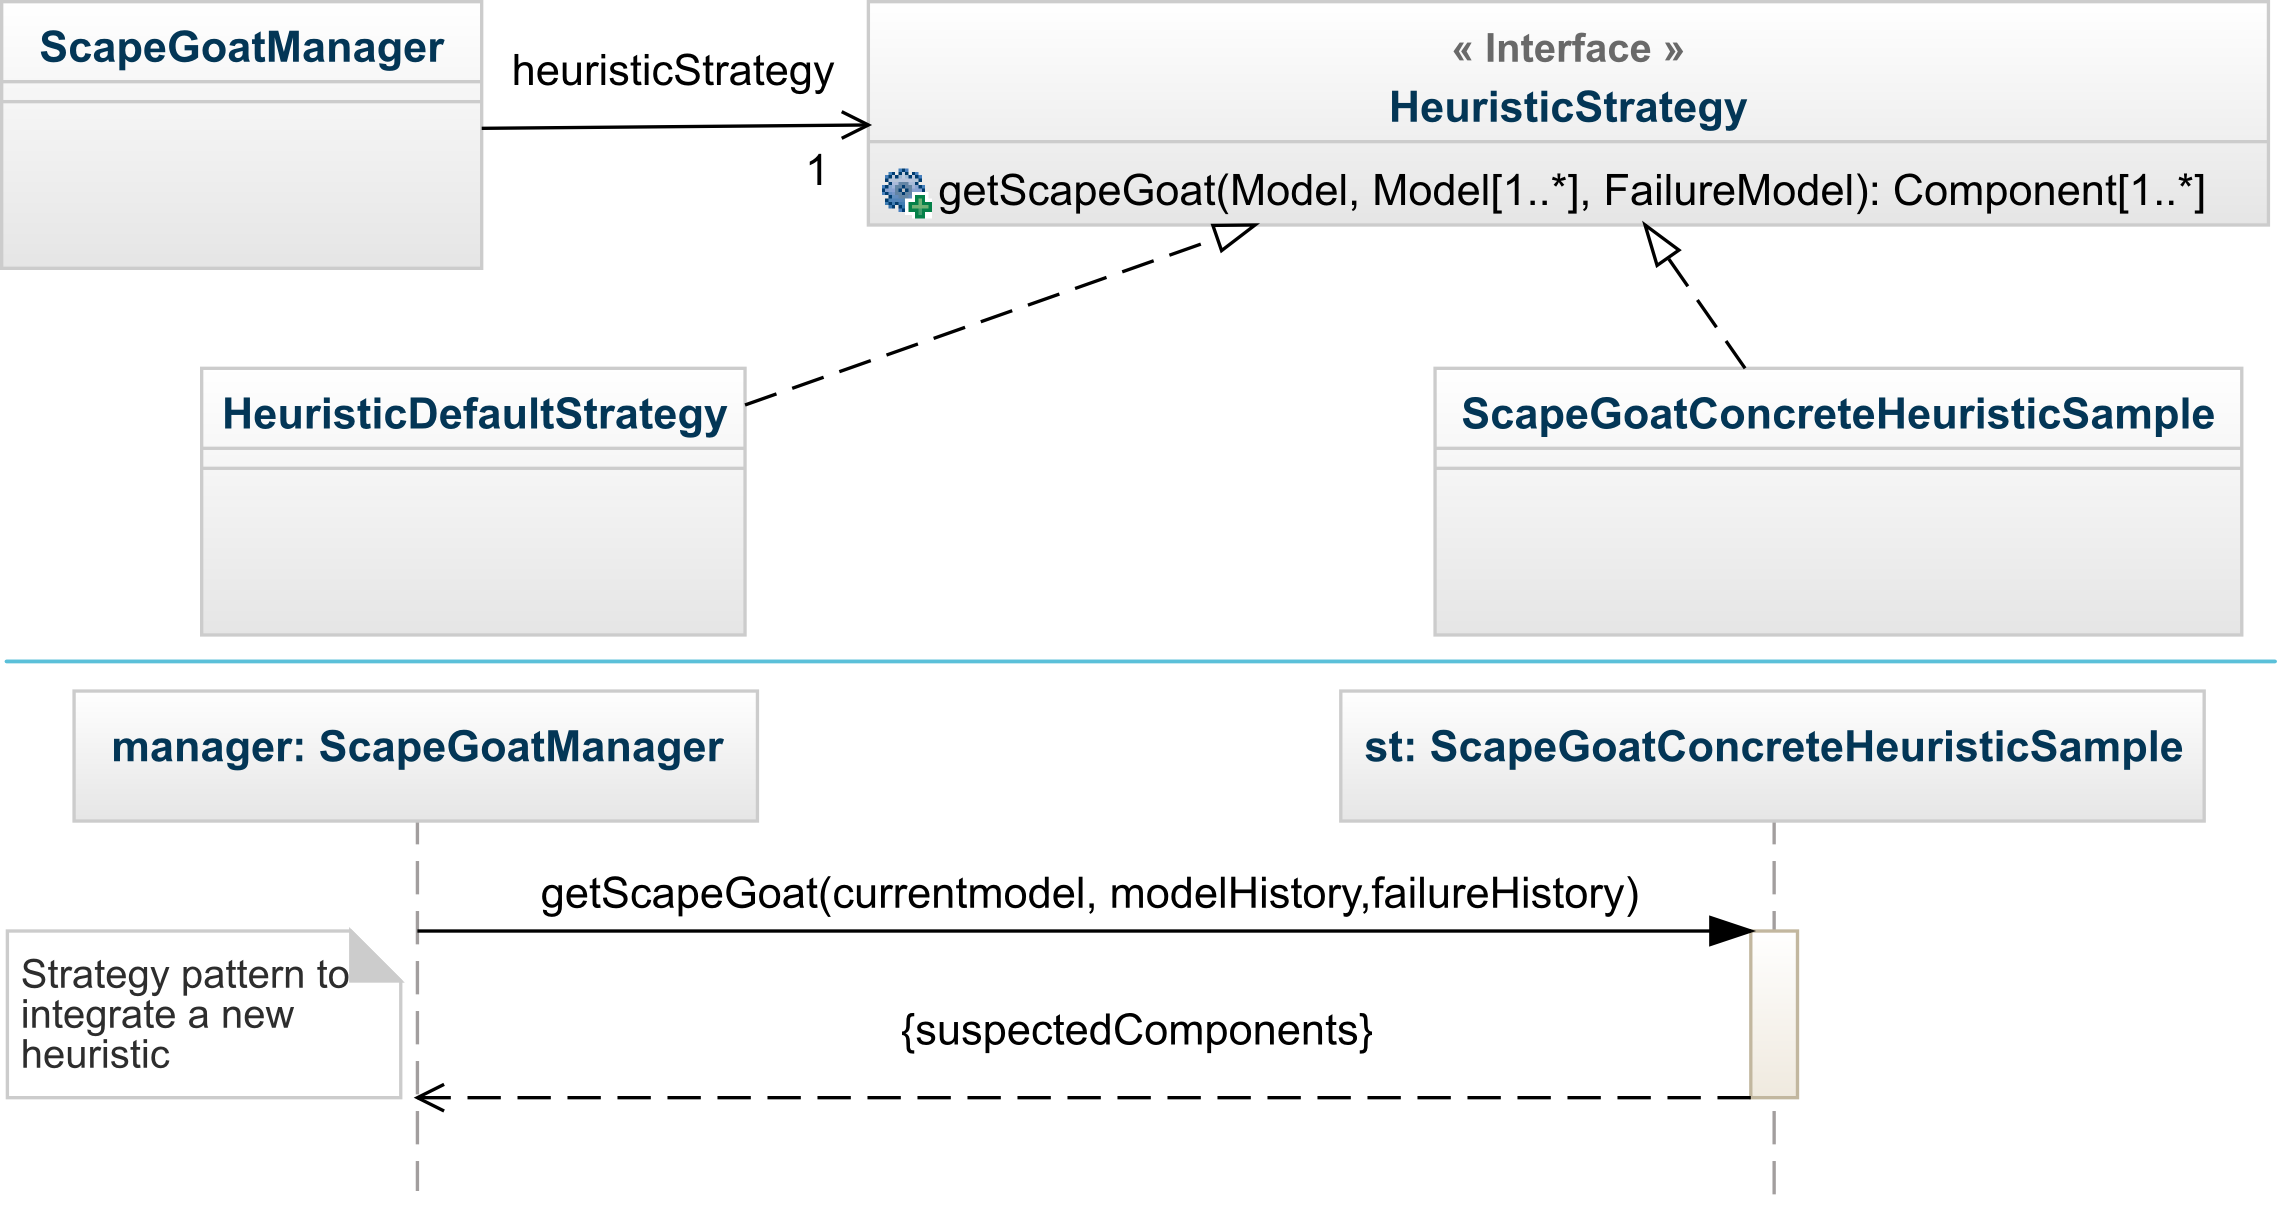
\includegraphics[width=0.9\textwidth]{chapter5/figures/strategy}
\caption{\label{fig:strategy}Scapegoat's extensibility}
\end{figure}

A second extensible aspect of the framework is the admission control system.
The framework provides an API to hook user-defined actions when new components are submitted for deployment.
Basic data describing the execution platform in terms of resource availability, information about the already deployed components and the new component's contract are sent to the user-defined admission control system.
On each request, the admission control system has to accept or refuse the new component.
In this paper, we are using an approach which check the theoretical availability of resources whenever a component is deployed, and accept the new component if the contract can fit in the remaining available resources.
ScapeGoat is meant to support other policies as, for instance, overcommitment.
 
A last element that can be specialized to user needs is the contracts semantic.
In section~\ref{componentcontract} we describe how we interpret the contract in this work.
However, it is possible to define other contract semantics, for instance, accepting values that are closed to the limit defined in the contract, or using fuzzy values instead of sharp values.
It is worth noting that modifying the semantic of the contract would likely involved redefining the domain-specific language to describe contract and also modifying the admission control system.

\subsubsection{Implementation strategy}
Scapegoat aims at minimizing monitoring overhead when the framework is running in \textit{Global Monitoring} mode. 
To achieve this, ScapeGoat removes as many monitoring probes as possible and only activates probes that are required.
This requires changing the bytecode that defines the application's classes at runtime, when the monitoring mode changes.
Bytecode is changed at a per-component basis.
We use the ASM library to perform bytecode manipulation and a Java agent to get access to and transform the classes.
Bytecode manipulation has been proposed before for resource accounting and profiling in Java \cite{binder_portable_2006,Binder200645,czajkowski_jres:_1998}.

The framework also proposes an on demand memory monitoring solution based on exploring the heap.
We built this solution on top of the JVM Tool Interface (JVMTI) by implementing the algorithms proposed in~\cite{Price:2003:GCM:829515.830545, Geoffray5270296}, with the main difference being that our solution works without modifying the garbage collector.
This makes our approach portable and allows it to work with different garbage collector implementations. 

\subsection{Leveraging Models@run.time to build an efficient monitoring framework}\label{sec:heuristic-based-on-modeling}

As presented in section \ref{monitorContainer}, our approach offers a dynamic way to activate and deactivate fine-grain localized monitoring.
We use a heuristic to determine which components are more likely to be faulty.
Suspected components are the first to be monitored.

Our framework can support different heuristics, which can be application or domain-specific.
In this paper we propose a heuristic that leverages the use of the Models@run.time approach to infer the faulty components.
The heuristic is based on the assumption that the cause of newly detected misbehavior in an application is likely to come from the most recent changes in the application.
This can be better understood as follows:
\begin{itemize}
\leftskip -.2in
  \item recently added or updated components are more likely to be the source of a faulty behaviour;
  \item components that directly interact with recently added or updated components are also suspected.
\end{itemize}

We argue that when a problem is detected it is probable that recent changes have led to this problem, or else, it would have likely occurred earlier.
If recently changed components are monitored and determined to be healthy, it is probable that the problem comes from direct interactions with those components.
Indeed, changes to interactions can reveal dormant issues with the components.
The algorithm used for ranking the components is presented in more detail in listing \ref{algo:heuristic}.
In practice, we leverage the architectural-based history of evolutions of the application, which is provided by the Models@run.time approach.


\begin{lstlisting}[escapeinside={(*}{*)},caption=The ranking algorithm (uses the model history for ranking).,label=algo:heuristic,float=!h]
ranker() : list<Component>
	visited = (*$\emptyset$*)
	ranking = {}
	for each model M (*$\in$*) History
		N = {c (*$\mid$*) c was added in M}
		Neighbors (*$ = \bigcup_{c \in N}{c.neighbors}$*)
		ranking.add N(*$\setminus$*)visited
		visited = visited (*$\cup$*) N
		SortedNeighbors = sort (Neighbors (*$\setminus$*) visited)
		ranking.add SortedNeighbors
		visited = visited (*$\cup$*) Neighbors
	return ranking
	
sort (S : Set<Component>) : list<Component>
	r = {}
	if (*$S \ne \emptyset$*)
		choose (*$b \mid b \in S$*) (*$\wedge$*) b is newer than any other element in S
		r.add b, sort (S(*$\setminus$*){b})
	return r
\end{lstlisting}
